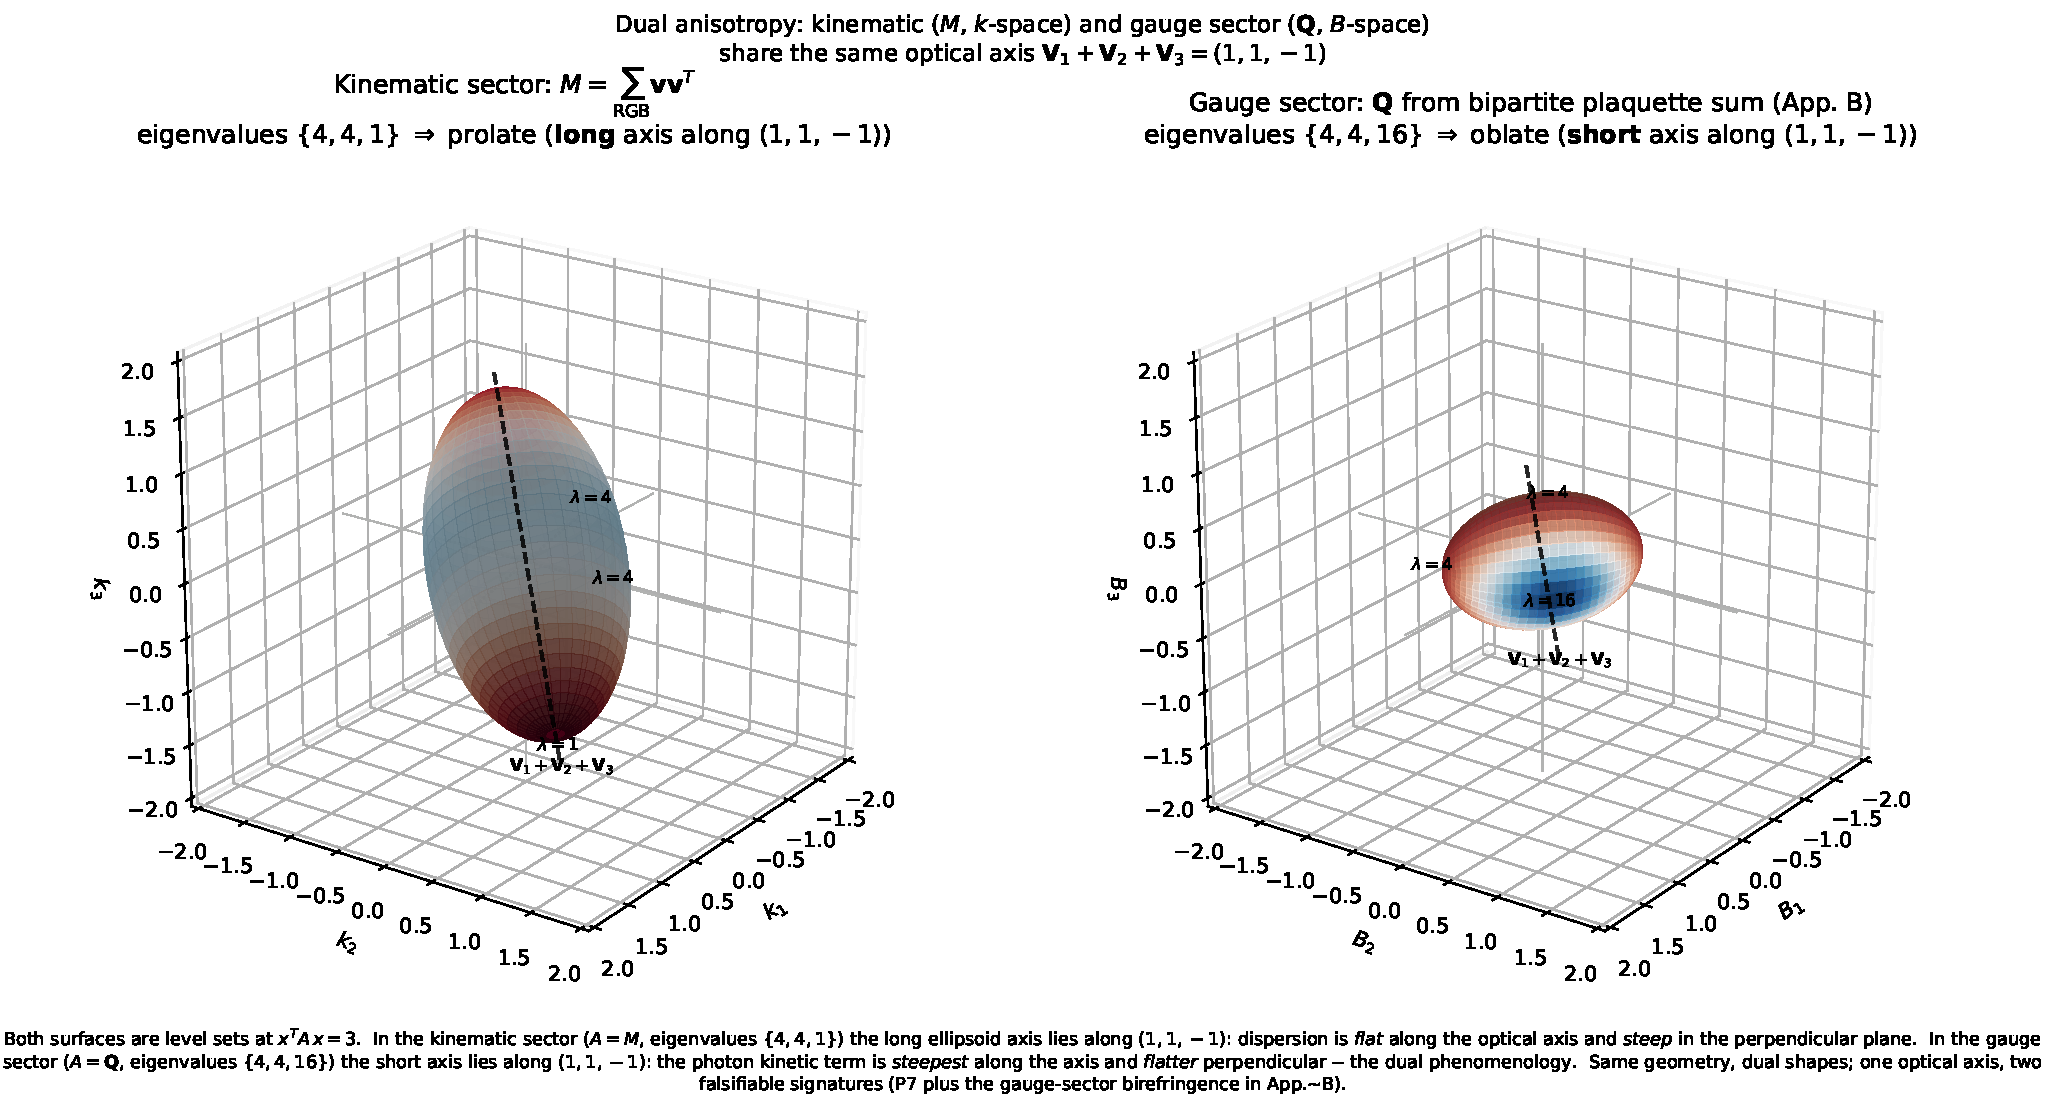
\includegraphics[width=\textwidth]{../figures/induced_action_ellipsoid}
\caption{Dual anisotropy on a single optical axis.
Both panels render level sets at $x^T A\,x = 3$ for the framework's two
anisotropy tensors; both share the special direction
$\mathbf{V}_1+\mathbf{V}_2+\mathbf{V}_3 = (1,1,-1)$ (dashed black line).
\textbf{Left (kinematic sector):} the frame matrix
$M = \sum_\mathrm{RGB}\mathbf{v}\mathbf{v}^T$
(Eq.~\ref{eq:frame_matrix}) on $\mathbf{k}$-space.  Eigenvalues
$\{4, 4, 1\}$ produce a \emph{prolate} ellipsoid whose \emph{long} axis
lies along the optical axis: kinematic dispersion is flat along
$(1,1,-1)$ and steep in the perpendicular plane.  This is the same
quadratic form that underlies the $|\tilde{H}_\text{RGB}|^2$ expansion
of $M_\text{eff}$ (Eq.~\ref{eq:M_eff},
Section~\ref{subsec:p7_photon_dispersion}).
\textbf{Right (gauge sector):} the bipartite plaquette tensor
$\mathbf{Q}$ (Eq.~\ref{eq:Q_matrix}) on $\mathbf{B}$-space (the Hodge
dual of antisymmetric $F_{ij}$).  Eigenvalues $\{4, 4, 16\}$ produce an
\emph{oblate} ellipsoid whose \emph{short} axis lies along $(1,1,-1)$:
the induced photon kinetic term is steepest along the optical axis and
flatter perpendicular --- the dual of the kinematic shape.  Both
anisotropies inherit the special direction from the same bipartite
RGB/CMY geometry; the dual ellipsoid shapes give two independent
falsifiable signatures with one optical axis (kinematic-sector birefringence
in P7, gauge-sector birefringence in Appendix~\ref{sec:induced_gauge_action}).}
\label{fig:induced_action_ellipsoid}
